\subsection{Construction de formules}
Le vocabulaire du langage de la logique propositionnelle est composé de :
\begin{enumerate}
  \item de propositions $x$, $y$, $z$, ...; ou $X$, $Y$, $Z$, ...;
  \item de deux constantes vrai ($\top$ ou $1$) et faux ($\bot$ ou $0$);
  \item d'un ensemble de connecteurs logiques : $\neg$, $\wedge$, $\vee$, $\rightarrow$, $\leftrightarrow$.
  \item de paranthèses $(\ )$.
\end{enumerate}


\subsection{Sémantique}
\begin{definition}{Sémantique}{sémantique}
La sémantique d'une formule est la valeur de vérité de cette formule. La valeur de vérité d'une formule
$\Phi$ formée àpd propositions d'un ensemble $X$, évaluée avec la fonction d'interprétation $V$, est notée $\llbracket \Phi \rrbracket_V$.
La fonction $\llbracket \Phi \rrbracket_V$ est définie par induction sur la syntaxe de $\Phi$ de la façon suivante :
\begin{itemize}[label=$\bullet$]
  \item $\llbracket \top\rrbracket_V = 1$ ; $\llbracket \bot\rrbracket_V = 0$ ; $\llbracket x\rrbracket_V = V(x)$
  \item $\llbracket \neg \Phi\rrbracket_V = 1 - \llbracket \Phi\rrbracket_V$
  \item $\llbracket \Phi_1 \vee \Phi_2\rrbracket_V = \text{max}(\llbracket\Phi_1\rrbracket_V,\llbracket\Phi_2\rrbracket_V)$
  \item $\llbracket \Phi_1 \land \Phi_2\rrbracket_V = \text{min}(\llbracket\Phi_1\rrbracket_V,\llbracket\Phi_2\rrbracket_V)$
  \item $\llbracket \Phi_1 \leftarrow \Phi_2\rrbracket_V = \text{max}(1 - \llbracket\Phi_1\rrbracket_V,\llbracket\Phi_2\rrbracket_V)$
  \item $\llbracket \Phi_1 \leftrightarrow \Phi_2\rrbracket_V = \text{min}(\llbracket\Phi_1\rightarrow\Phi_2\rrbracket_V,\llbracket\Phi_2\rightarrow\Phi_1\rrbracket_V)$
\end{itemize}
Nous notons $V\vDash\Phi\Leftrightarrow\llbracket\Phi\rrbracket_V=1$ soit "$V$ satisfait $\Phi$."
\end{definition}

L'information contenue dans la définition est souvent représentée sous forme de table de verité : 
\begin{center}
  \begin{tabular}{|c|c|c|c|c|c|}
    \hline 
    $\Phi_1$ & $\Phi_2$ & $\Phi_1\vee\Phi_2$ & $\Phi_1\wedge\Phi_2$ & $\Phi_1\rightarrow\Phi_2$ & $\Phi_1\leftrightarrow\Phi_2$ \\ 
    \hline 
    0 & 0 & 0 & 0 & 1 & 1 \\ 
    \hline 
    0 & 1 & 1 & 0 & 1 & 0 \\ 
    \hline 
    1 & 0 & 1 & 0 & 0 & 0 \\ 
    \hline 
    1 & 1 & 1 & 1 & 1 & 1 \\ 
    \hline 
  \end{tabular}
\end{center}
\warningbox{Dans l'implication suivante : $\Phi_1\rightarrow\Phi_2$, la cas où $\Phi_1$ est faux ne nous intéresse pas. Dans ce cas, l'implication est toujours vraie.}



\subsection{Validité et Stabilité}
\subsubsection{Définitions}
\begin{definition}{Formule propositionnelle satisfaisable}{formule_propositionnelle_satisfaisable}
Une formule propositionnelle $\Phi$ est \textbf{satisfaisable} $\Leftrightarrow$ il existe une fonction d'interprétation $V$ pour les propositions de $\Phi$, telle que 
$V\vDash\Phi$.
\end{definition}
\begin{definition}{Formule propositionnelle valide}{formule_propositionnelle_valide}
Une formule propositionnelle $\Phi$ est \textbf{valide} $\Leftrightarrow$ pour toute fonction d'interprétation $V$ pour les propositions de $\Phi$, $V\vDash\Phi$.
\end{definition}

\subsubsection{Conséquence logique}
\begin{definition}{Conséquence Logique}{conséquence_logique}
Soit $\Phi_1,...,\Phi_n,\Phi$ des formules. On dira que $\Phi$ est une \textbf{conséquence logique} de $\Phi_1,...,\Phi_n$, noté $\Phi_1,...,\Phi_n\vDash\Phi$, si ($\Phi_1\land ...\land\Phi_n$)$\rightarrow\Phi$ est valide.
\end{definition}

\subsubsection{Equivalence}

\begin{definition}{Formules équivalentes}{formules_équivalentes}
Deux formules, $\Phi$ et $\Psi$, sont \textbf{équivalentes} si la formule $\Phi\leftrightarrow\Psi$ est valide. On notera $\Phi\equiv\Psi$.
\end{definition}
Pour toutes formules $\Phi_1,\Phi_2,\Phi_3$ :
\begin{itemize}[label=$\bullet$]
  \item $\neg\neg\Phi_1\equiv\Phi_1$
  \item $\neg(\Phi_1\land\Phi_2)\equiv(\neg\Phi_1\lor\neg\Phi_2)$
  \item $\neg(\Phi_1\lor\Phi_2)\equiv(\neg\Phi_1\land\neg\Phi_2)$
  \item $\Phi_1\land(\Phi_2\lor\Phi_3)\equiv(\Phi_1\land\Phi_2)\lor(\Phi_1\land\Phi_3)$
  \item $\Phi_1\lor(\Phi_2\land\Phi_3)\equiv(\Phi_1\lor\Phi_2)\land(\Phi_1\lor\Phi_3)$
  \item $\Phi_1\rightarrow\Phi_2\equiv(\neg\Phi_1\lor\Phi_2)$
\end{itemize}

\subsubsection{Lien entre satisfaisabilité et validité}
\begin{theorem}{Lien entre satisfaisabilité et validité}{lien_satisfaisabilité_validité}
  Une formule $\Phi$ est valide $\Leftrightarrow$ $\neg\Phi$ est insatisfaisable.
\end{theorem}
\begin{figure}[H]
  \centering
  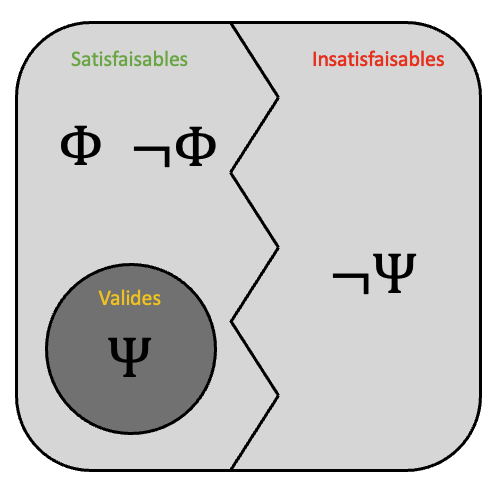
\includegraphics[scale=0.3]{pictures/satisf:vali.png}
  \caption{Lien entre satisfaisabilité et validité}
\end{figure}


\subsubsection{Tableaux sémantiques}
\begin{definition}{Littéral}{littéral}
  Un littéral est une proposition $x$ ou la négation d'une proposition $\neg x$.
\end{definition}
La méthode des tableaux sémantiques est un algorithme pour tester la satisfaisabilité d'une formule. Elle consiste à construire un arbre dont les noeuds sont des formules et les feuilles sont des littéraux. On construit l'arbre de la façon suivante :
\begin{itemize}[label=$\bullet$]
  \item On place la formule à tester à la racine de l'arbre.
  \item On applique les règles suivantes jusqu'à ce que l'arbre soit complet :
  \begin{itemize}[label=$\circ$]
    \item Si la formule à tester est une constante, on arrête.
    \item Si la formule à tester est une conjonction, on ajoute les deux conjoncteurs comme fils de la formule à tester.
    \item Si la formule à tester est une disjonction, on ajoute un fils avec le premier disjoncteur et un autre fils avec le deuxième disjoncteur.
    \item Si la formule à tester est une implication, on ajoute un fils avec la négation de l'antécédent et un autre fils avec le conséquent.
    \item Si la formule à tester est une équivalence, on ajoute un fils avec la négation de la première formule et un autre fils avec la deuxième formule.
    \item Si la formule à tester est une négation, on ajoute un fils avec la négation de la formule à tester.
  \end{itemize}
\end{itemize}
\begin{remark}
  TODO --> Vérifier l'algorithme
\end{remark}